% Options for packages loaded elsewhere
\PassOptionsToPackage{unicode}{hyperref}
\PassOptionsToPackage{hyphens}{url}
%
\documentclass[
  12pt,
  a4paper,
  DIV=11,
  numbers=noendperiod]{scrreprt}

\usepackage{amsmath,amssymb}
\usepackage{setspace}
\usepackage{iftex}
\ifPDFTeX
  \usepackage[T1]{fontenc}
  \usepackage[utf8]{inputenc}
  \usepackage{textcomp} % provide euro and other symbols
\else % if luatex or xetex
  \usepackage{unicode-math}
  \defaultfontfeatures{Scale=MatchLowercase}
  \defaultfontfeatures[\rmfamily]{Ligatures=TeX,Scale=1}
\fi
\usepackage{lmodern}
\ifPDFTeX\else  
    % xetex/luatex font selection
\fi
% Use upquote if available, for straight quotes in verbatim environments
\IfFileExists{upquote.sty}{\usepackage{upquote}}{}
\IfFileExists{microtype.sty}{% use microtype if available
  \usepackage[]{microtype}
  \UseMicrotypeSet[protrusion]{basicmath} % disable protrusion for tt fonts
}{}
\usepackage{xcolor}
\setlength{\emergencystretch}{3em} % prevent overfull lines
\setcounter{secnumdepth}{5}
% Make \paragraph and \subparagraph free-standing
\makeatletter
\ifx\paragraph\undefined\else
  \let\oldparagraph\paragraph
  \renewcommand{\paragraph}{
    \@ifstar
      \xxxParagraphStar
      \xxxParagraphNoStar
  }
  \newcommand{\xxxParagraphStar}[1]{\oldparagraph*{#1}\mbox{}}
  \newcommand{\xxxParagraphNoStar}[1]{\oldparagraph{#1}\mbox{}}
\fi
\ifx\subparagraph\undefined\else
  \let\oldsubparagraph\subparagraph
  \renewcommand{\subparagraph}{
    \@ifstar
      \xxxSubParagraphStar
      \xxxSubParagraphNoStar
  }
  \newcommand{\xxxSubParagraphStar}[1]{\oldsubparagraph*{#1}\mbox{}}
  \newcommand{\xxxSubParagraphNoStar}[1]{\oldsubparagraph{#1}\mbox{}}
\fi
\makeatother


\providecommand{\tightlist}{%
  \setlength{\itemsep}{0pt}\setlength{\parskip}{0pt}}\usepackage{longtable,booktabs,array}
\usepackage{calc} % for calculating minipage widths
% Correct order of tables after \paragraph or \subparagraph
\usepackage{etoolbox}
\makeatletter
\patchcmd\longtable{\par}{\if@noskipsec\mbox{}\fi\par}{}{}
\makeatother
% Allow footnotes in longtable head/foot
\IfFileExists{footnotehyper.sty}{\usepackage{footnotehyper}}{\usepackage{footnote}}
\makesavenoteenv{longtable}
\usepackage{graphicx}
\makeatletter
\newsavebox\pandoc@box
\newcommand*\pandocbounded[1]{% scales image to fit in text height/width
  \sbox\pandoc@box{#1}%
  \Gscale@div\@tempa{\textheight}{\dimexpr\ht\pandoc@box+\dp\pandoc@box\relax}%
  \Gscale@div\@tempb{\linewidth}{\wd\pandoc@box}%
  \ifdim\@tempb\p@<\@tempa\p@\let\@tempa\@tempb\fi% select the smaller of both
  \ifdim\@tempa\p@<\p@\scalebox{\@tempa}{\usebox\pandoc@box}%
  \else\usebox{\pandoc@box}%
  \fi%
}
% Set default figure placement to htbp
\def\fps@figure{htbp}
\makeatother

\usepackage{indentfirst}
\usepackage{float}
\floatplacement{figure}{H}
\IfFileExists{plex-otf.sty}{
  %% Full TeXlive
  \usepackage[
    % math,
    RM={Scale=0.94},SS={Scale=0.94},SScon={Scale=0.94},TT={Scale=MatchLowercase,FakeStretch=0.9},
    DefaultFeatures={Ligatures=Common}
  ]{plex-otf}
  % \usepackage[Scale=MatchUppercase]{juliamono}
}{
  %% TinyTeX
  \usepackage{libertine}
}
\KOMAoption{captions}{tableheading}
\makeatletter
\@ifpackageloaded{caption}{}{\usepackage{caption}}
\AtBeginDocument{%
\ifdefined\contentsname
  \renewcommand*\contentsname{Содержание}
\else
  \newcommand\contentsname{Содержание}
\fi
\ifdefined\listfigurename
  \renewcommand*\listfigurename{Список иллюстраций}
\else
  \newcommand\listfigurename{Список иллюстраций}
\fi
\ifdefined\listtablename
  \renewcommand*\listtablename{Список таблиц}
\else
  \newcommand\listtablename{Список таблиц}
\fi
\ifdefined\figurename
  \renewcommand*\figurename{Рисунок}
\else
  \newcommand\figurename{Рисунок}
\fi
\ifdefined\tablename
  \renewcommand*\tablename{Таблица}
\else
  \newcommand\tablename{Таблица}
\fi
}
\@ifpackageloaded{float}{}{\usepackage{float}}
\floatstyle{ruled}
\@ifundefined{c@chapter}{\newfloat{codelisting}{h}{lop}}{\newfloat{codelisting}{h}{lop}[chapter]}
\floatname{codelisting}{Список}
\newcommand*\listoflistings{\listof{codelisting}{Листинги}}
\makeatother
\makeatletter
\makeatother
\makeatletter
\@ifpackageloaded{caption}{}{\usepackage{caption}}
\@ifpackageloaded{subcaption}{}{\usepackage{subcaption}}
\makeatother

\ifLuaTeX
\usepackage[bidi=basic]{babel}
\else
\usepackage[bidi=default]{babel}
\fi
\babelprovide[main,import]{russian}
\babelprovide[import]{english}
% get rid of language-specific shorthands (see #6817):
\let\LanguageShortHands\languageshorthands
\def\languageshorthands#1{}
\usepackage[style=gost-numeric,backend=biber,langhook=extras,autolang=other*]{biblatex}
\addbibresource{bib/cite.bib}
\usepackage{csquotes}
\usepackage{bookmark}

\IfFileExists{xurl.sty}{\usepackage{xurl}}{} % add URL line breaks if available
\urlstyle{same} % disable monospaced font for URLs
\hypersetup{
  pdftitle={Отчёт по лабораторной работе №1},
  pdfauthor={Пакавира Арсениу Висенте Луиш},
  pdflang={ru-RU},
  hidelinks,
  pdfcreator={LaTeX via pandoc}}


\title{Отчёт по лабораторной работе №1}
\usepackage{etoolbox}
\makeatletter
\providecommand{\subtitle}[1]{% add subtitle to \maketitle
  \apptocmd{\@title}{\par {\large #1 \par}}{}{}
}
\makeatother
\subtitle{Дисциплина: Администрирование сетевых подсистем}
\author{Пакавира Арсениу Висенте Луиш}
\date{}

\begin{document}
\maketitle

\renewcommand*\contentsname{Содержание}
{
\setcounter{tocdepth}{1}
\tableofcontents
}
\listoffigures
\listoftables

\setstretch{1.5}
\chapter{Цель
работы}\label{ux446ux435ux43bux44c-ux440ux430ux431ux43eux442ux44b}

Целью данной работы является приобретение практических навыков установки
Rocky Linux на виртуальную машину с помощью инструмента Vagrant.

\chapter{Выполнение лабораторной
работы}\label{ux432ux44bux43fux43eux43bux43dux435ux43dux438ux435-ux43bux430ux431ux43eux440ux430ux442ux43eux440ux43dux43eux439-ux440ux430ux431ux43eux442ux44b}

В рабочем каталоге ОС Windows созданы подкаталоги
\texttt{C:\textbackslash{}work\textbackslash{}bahis\textbackslash{}packer}
и
\texttt{C:\textbackslash{}work\textbackslash{}user\textbackslash{}vagrant},
предназначенные для подготовки box-файла Vagrant (\textbf{?@fig-1}). В
каталоге \texttt{packer} размещены образ Rocky-9.4-x86\_64-minimal.iso,
исполняемый файл packer.exe, файл конфигурации vagrant-rocky.pkr.hcl и
подкаталог \texttt{http}, что соответствует требованиям к структуре
проекта (\textbf{?@fig-2}).


\includegraphics[width=0.7\linewidth,height=\textheight,keepaspectratio]{image/1.png}
\href{https://github.com/ArsenioPacavira99/study_2025-2026_net-os-admin-12/tree/master/labs/lab01/report/image/1.png}{рис.
1}


\includegraphics[width=0.7\linewidth,height=\textheight,keepaspectratio]{image/2.png}
\href{https://github.com/ArsenioPacavira99/study_2025-2026_net-os-admin-12/tree/master/labs/lab01/report/image/2.png}{рис.
2}

Файл \texttt{vagrant-rocky.pkr.hcl} содержит блок \texttt{packer} с
разделом \texttt{required\_plugins} (vagrant, virtualbox), а также
переменные, определяющие версию дистрибутива, размер диска, контрольную
сумму ISO-образа, архитектуру и параметры SSH (\textbf{?@fig-3}). В
подкаталоге \texttt{http} размещён файл \texttt{ks.cfg}, задающий
автоматизированные параметры установки системы: загрузчик, очистку
разделов, язык, сетевые настройки (DHCP), создание пользователя и
post-настройки (\textbf{?@fig-4}).


\includegraphics[width=0.7\linewidth,height=\textheight,keepaspectratio]{image/3.png}
\href{https://github.com/ArsenioPacavira99/study_2025-2026_net-os-admin-12/tree/master/labs/lab01/report/image/3.png}{рис.
3}


\includegraphics[width=0.7\linewidth,height=\textheight,keepaspectratio]{image/4.png}
\href{https://github.com/ArsenioPacavira99/study_2025-2026_net-os-admin-12/tree/master/labs/lab01/report/image/4.png}{рис.
4}

В каталоге \texttt{vagrant} размещён файл \texttt{Vagrantfile},
определяющий конфигурацию виртуальной машины server: имя box
\texttt{rocky9}, сетевой интерфейс с IP 192.168.1.1, параметры
VirtualBox (RAM, CPU, VRAM, графический контроллер) и подключение
provision-скриптов (\textbf{?@fig-5}). Также создан каталог
\texttt{provision} с подкаталогами \texttt{default}, \texttt{server} и
\texttt{client}, предназначенными для разделения сценариев настройки
окружения (\textbf{?@fig-6}).


\includegraphics[width=0.7\linewidth,height=\textheight,keepaspectratio]{image/5.png}
\href{https://github.com/ArsenioPacavira99/study_2025-2026_net-os-admin-12/tree/master/labs/lab01/report/image/5.png}{рис.
5}


\includegraphics[width=0.7\linewidth,height=\textheight,keepaspectratio]{image/6.png}
\href{https://github.com/ArsenioPacavira99/study_2025-2026_net-os-admin-12/tree/master/labs/lab01/report/image/6.png}{рис.
6}

В подкаталогах \texttt{default}, \texttt{server} и \texttt{client}
размещены скрипты-заглушки \texttt{01-dummy.sh}, выводящие сообщение о
выполнении provisioning (\textbf{?@fig-7}). В каталоге \texttt{default}
дополнительно размещены скрипты \texttt{01-user.sh} (создание
пользователя bahis, добавление в группу wheel, настройка PS1) и
\texttt{01-hostname.sh} (установка FQDN вида *.bahis.net)
(\textbf{?@fig-8}, \textbf{?@fig-9}). В каталоге \texttt{server}
размещён скрипт \texttt{02-forward.sh}, активирующий IP-маршрутизацию и
masquerading через firewalld, а в каталоге \texttt{client} --- скрипт
\texttt{01-routing.sh}, настраивающий шлюз 192.168.1.1 и параметры
интерфейсов через nmcli (\textbf{?@fig-10}, \textbf{?@fig-11}).


\includegraphics[width=0.7\linewidth,height=\textheight,keepaspectratio]{image/7.png}
\href{https://github.com/ArsenioPacavira99/study_2025-2026_net-os-admin-12/tree/master/labs/lab01/report/image/7.png}{рис.
7}

!{[}Скрипты-заглушки 01-dummy.sh в каталогах default, server и client{]}

!{[}Скрипты-заглушки 01-dummy.sh в каталогах default, server и client{]}


\includegraphics[width=0.7\linewidth,height=\textheight,keepaspectratio]{image/8.png}
\href{https://github.com/ArsenioPacavira99/study_2025-2026_net-os-admin-12/tree/master/labs/lab01/report/image/8.png}{рис.
8}


\includegraphics[width=0.7\linewidth,height=\textheight,keepaspectratio]{image/9.png}
\href{https://github.com/ArsenioPacavira99/study_2025-2026_net-os-admin-12/tree/master/labs/lab01/report/image/9.png}{рис.
9}


\includegraphics[width=0.7\linewidth,height=\textheight,keepaspectratio]{image/10.png}
\href{https://github.com/ArsenioPacavira99/study_2025-2026_net-os-admin-12/tree/master/labs/lab01/report/image/10.png}{рис.
10}


\includegraphics[width=0.7\linewidth,height=\textheight,keepaspectratio]{image/11.png}
\href{https://github.com/ArsenioPacavira99/study_2025-2026_net-os-admin-12/tree/master/labs/lab01/report/image/11.png}{рис.
11}

\chapter{Развёртывание лабораторного стенда на ОС
Windows}\label{ux440ux430ux437ux432ux451ux440ux442ux44bux432ux430ux43dux438ux435-ux43bux430ux431ux43eux440ux430ux442ux43eux440ux43dux43eux433ux43e-ux441ux442ux435ux43dux434ux430-ux43dux430-ux43eux441-windows}

В рабочем каталоге
\texttt{C:\textbackslash{}work\textbackslash{}user\textbackslash{}packer}
выполнены команды \texttt{packer.exe\ init\ vagrant-rocky.pkr.hcl} и
\texttt{packer.exe\ build\ vagrant-rocky.pkr.hcl}, в результате чего
произведена автоматическая установка Rocky Linux в VirtualBox и
сформирован box-файл (\textbf{?@fig-12}). По завершении сборки в
каталоге создан файл \texttt{vagrant-virtualbox-rocky-9-x86\_64.box},
подтверждающий корректное формирование образа для Vagrant
(\textbf{?@fig-13}).


\includegraphics[width=0.7\linewidth,height=\textheight,keepaspectratio]{image/12.png}
\href{https://github.com/ArsenioPacavira99/study_2025-2026_net-os-admin-12/tree/master/labs/lab01/report/image/12.png}{рис.
12}


\includegraphics[width=0.7\linewidth,height=\textheight,keepaspectratio]{image/13.png}
\href{https://github.com/ArsenioPacavira99/study_2025-2026_net-os-admin-12/tree/master/labs/lab01/report/image/13.png}{рис.
13}

Далее выполнена регистрация образа в Vagrant командой
\texttt{vagrant\ box\ add\ rocky9\ vagrant-virtualbox-rocky-9-x86\_64.box},
после чего box добавлен под именем \texttt{rocky9} (\textbf{?@fig-14}).
Запуск виртуальной машины Server осуществлён командой
\texttt{vagrant\ up\ server}, выполнена инициализация сетевых
интерфейсов, проброс портов и запуск provisioning-сценариев
(\textbf{?@fig-15}).


\includegraphics[width=0.7\linewidth,height=\textheight,keepaspectratio]{image/14.png}
\href{https://github.com/ArsenioPacavira99/study_2025-2026_net-os-admin-12/tree/master/labs/lab01/report/image/14.png}{рис.
14}


\includegraphics[width=0.7\linewidth,height=\textheight,keepaspectratio]{image/15.png}
\href{https://github.com/ArsenioPacavira99/study_2025-2026_net-os-admin-12/tree/master/labs/lab01/report/image/15.png}{рис.
15}

Запуск виртуальной машины Client выполнен командой
\texttt{vagrant\ up\ client}, произведена настройка сетевых адаптеров и
подключение через SSH (\textbf{?@fig-16}). В графическом интерфейсе
VirtualBox обе виртуальные машины успешно загружены, выполнен вход под
пользователем \texttt{vagrant} с паролем \texttt{vagrant}
(\textbf{?@fig-17}, \textbf{?@fig-17-1}).


\includegraphics[width=0.7\linewidth,height=\textheight,keepaspectratio]{image/16.png}
\href{https://github.com/ArsenioPacavira99/study_2025-2026_net-os-admin-12/tree/master/labs/lab01/report/image/16.png}{рис.
16}


\includegraphics[width=0.7\linewidth,height=\textheight,keepaspectratio]{image/17.png}
\href{https://github.com/ArsenioPacavira99/study_2025-2026_net-os-admin-12/tree/master/labs/lab01/report/image/17.png}{рис.
17}

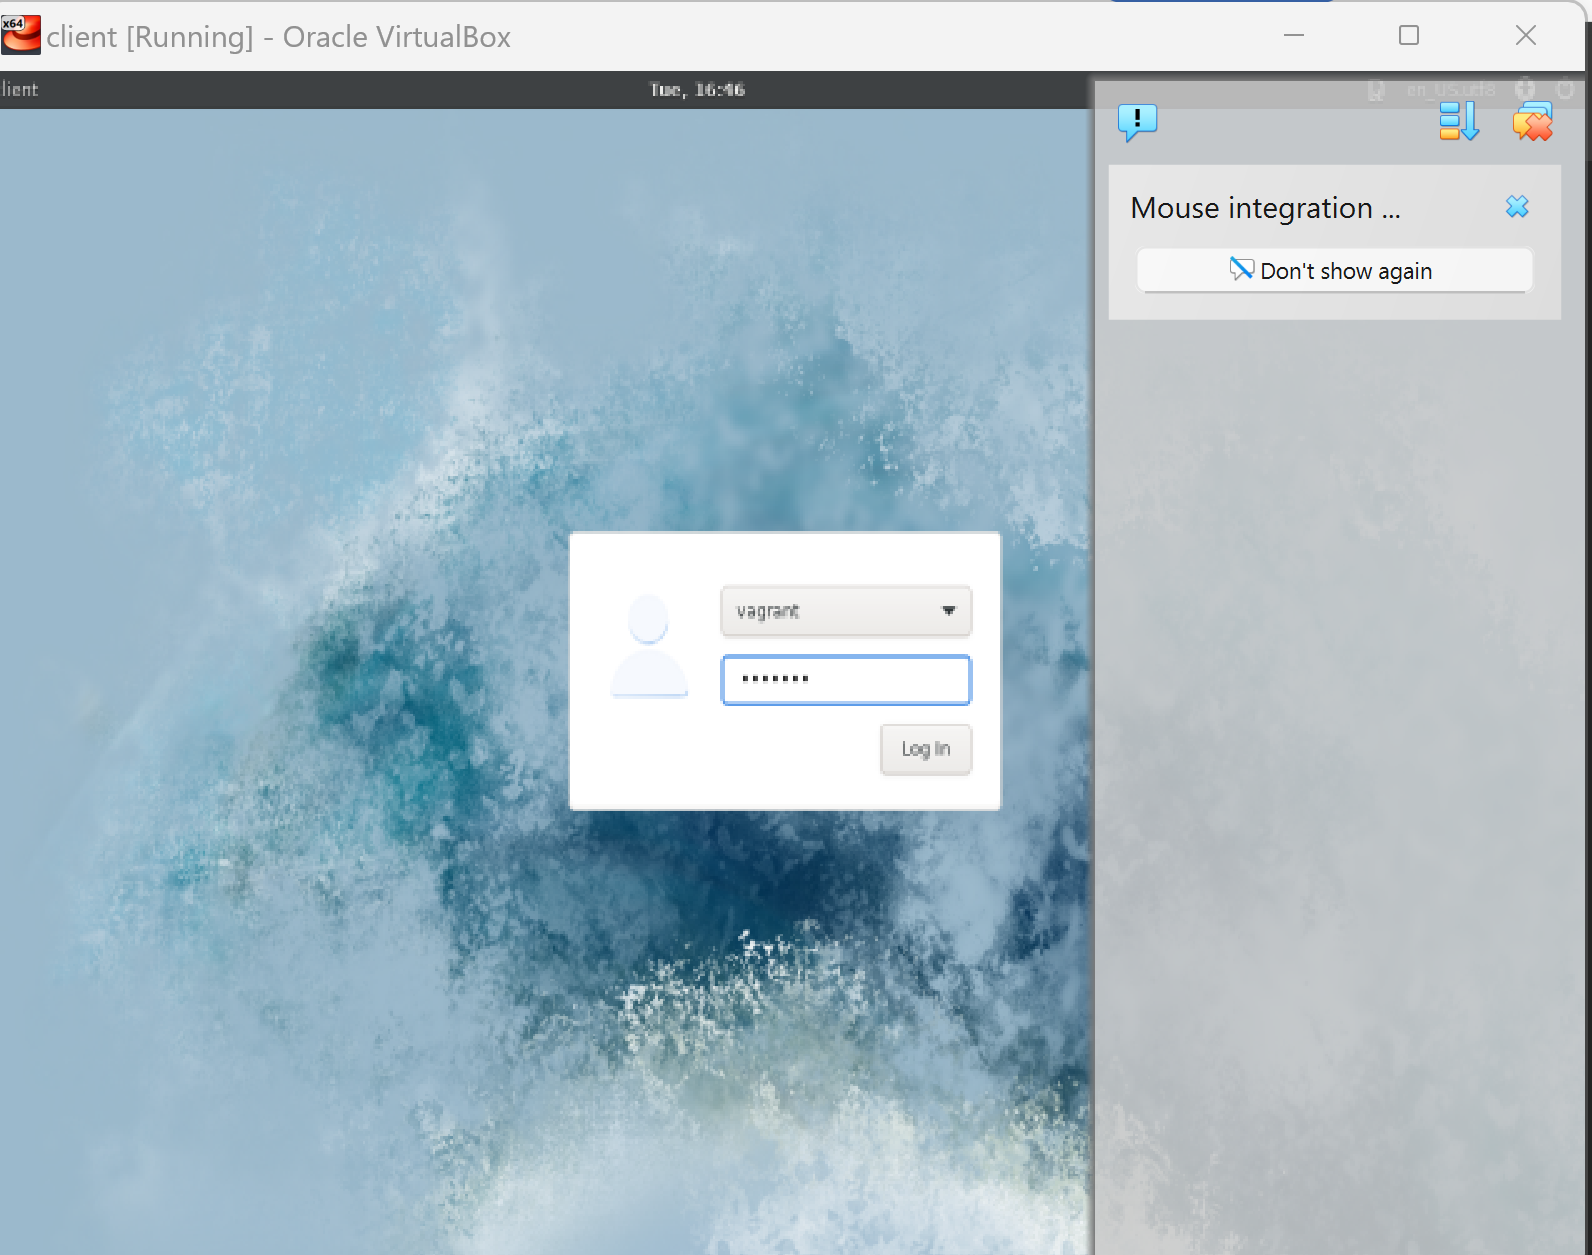
\includegraphics[width=0.7\linewidth,height=\textheight,keepaspectratio]{image/17-1.png}
\href{https://github.com/ArsenioPacavira99/study_2025-2026_net-os-admin-12/tree/master/labs/lab01/report/image/17-1.png}{рис.
17-1}

Подключение к серверу выполнено командой \texttt{vagrant\ ssh\ server},
после ввода пароля осуществлён переход к пользователю \texttt{bahis}
командой \texttt{su\ -\ bahis} и последующий выход из сеанса
(\textbf{?@fig-18}). Аналогичные действия выполнены для клиента с
использованием команды \texttt{vagrant\ ssh\ client}
(\textbf{?@fig-18-1}).


\includegraphics[width=0.7\linewidth,height=\textheight,keepaspectratio]{image/18.png}
\href{https://github.com/ArsenioPacavira99/study_2025-2026_net-os-admin-12/tree/master/labs/lab01/report/image/18.png}{рис.
18}

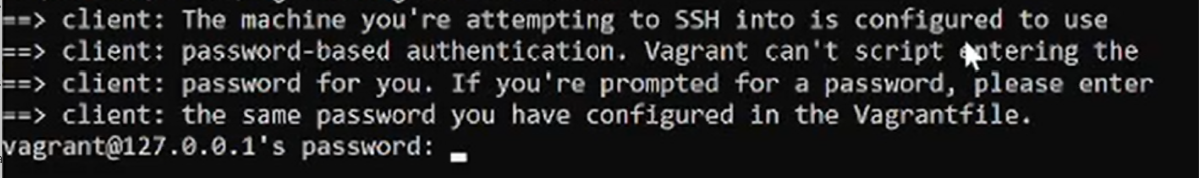
\includegraphics[width=0.7\linewidth,height=\textheight,keepaspectratio]{image/18-1.png}
\href{https://github.com/ArsenioPacavira99/study_2025-2026_net-os-admin-12/tree/master/labs/lab01/report/image/18-1.png}{рис.
18-1}

Завершение работы лабораторного стенда выполнено командами
\texttt{vagrant\ halt\ server} и \texttt{vagrant\ halt\ client}, что
обеспечило корректное выключение обеих виртуальных машин
(\textbf{?@fig-19}).


\includegraphics[width=0.7\linewidth,height=\textheight,keepaspectratio]{image/19.png}
\href{https://github.com/ArsenioPacavira99/study_2025-2026_net-os-admin-12/tree/master/labs/lab01/report/image/19.png}{рис.
19}

\chapter{Внесение изменений в настройки внутреннего окружения
виртуальной
машины}\label{ux432ux43dux435ux441ux435ux43dux438ux435-ux438ux437ux43cux435ux43dux435ux43dux438ux439-ux432-ux43dux430ux441ux442ux440ux43eux439ux43aux438-ux432ux43dux443ux442ux440ux435ux43dux43dux435ux433ux43e-ux43eux43aux440ux443ux436ux435ux43dux438ux44f-ux432ux438ux440ux442ux443ux430ux43bux44cux43dux43eux439-ux43cux430ux448ux438ux43dux44b}

В конфигурационном файле \texttt{Vagrantfile} перед разделом с описанием
виртуальной машины server добавлены provisioning-блоки
\texttt{common\ user} и \texttt{common\ hostname}, обеспечивающие
выполнение скриптов \texttt{01-user.sh} и \texttt{01-hostname.sh} при
загрузке ВМ (\textbf{?@fig-20}). Это гарантирует создание пользователя
user и установку доменного имени вида \texttt{*.user.net}.


\includegraphics[width=0.7\linewidth,height=\textheight,keepaspectratio]{image/20.png}
\href{https://github.com/ArsenioPacavira99/study_2025-2026_net-os-admin-12/tree/master/labs/lab01/report/image/20.png}{рис.
20}

Для применения изменений выполнены команды
\texttt{vagrant\ up\ server\ -\/-provision} и
\texttt{vagrant\ up\ client\ -\/-provision}, в результате чего повторно
запущены provisioning-сценарии и зафиксированы внутренние настройки
виртуальных машин (\textbf{?@fig-21}, \textbf{?@fig-22}). В процессе
выполнения на сервере зафиксировано существование пользователя user, что
подтверждает корректную работу скрипта создания пользователя.


\includegraphics[width=0.7\linewidth,height=\textheight,keepaspectratio]{image/21.png}
\href{https://github.com/ArsenioPacavira99/study_2025-2026_net-os-admin-12/tree/master/labs/lab01/report/image/21.png}{рис.
21}


\includegraphics[width=0.7\linewidth,height=\textheight,keepaspectratio]{image/22.png}
\href{https://github.com/ArsenioPacavira99/study_2025-2026_net-os-admin-12/tree/master/labs/lab01/report/image/22.png}{рис.
22}

После применения настроек выполнен вход в графическом интерфейсе под
пользователем user на сервере и клиенте (\textbf{?@fig-23},
\textbf{?@fig-23-1}). При подключении по SSH командой
\texttt{vagrant\ ssh} выполнен переход к пользователю \texttt{user}
через \texttt{su\ -\ user}, при этом приглашение терминала отображается
в формате \texttt{user@server.usernet} и \texttt{user@client.user.net},
что подтверждает корректную настройку hostname и пользовательского
окружения (\textbf{?@fig-24}).


\includegraphics[width=0.7\linewidth,height=\textheight,keepaspectratio]{image/23.png}
\href{https://github.com/ArsenioPacavira99/study_2025-2026_net-os-admin-12/tree/master/labs/lab01/report/image/23.png}{рис.
23}

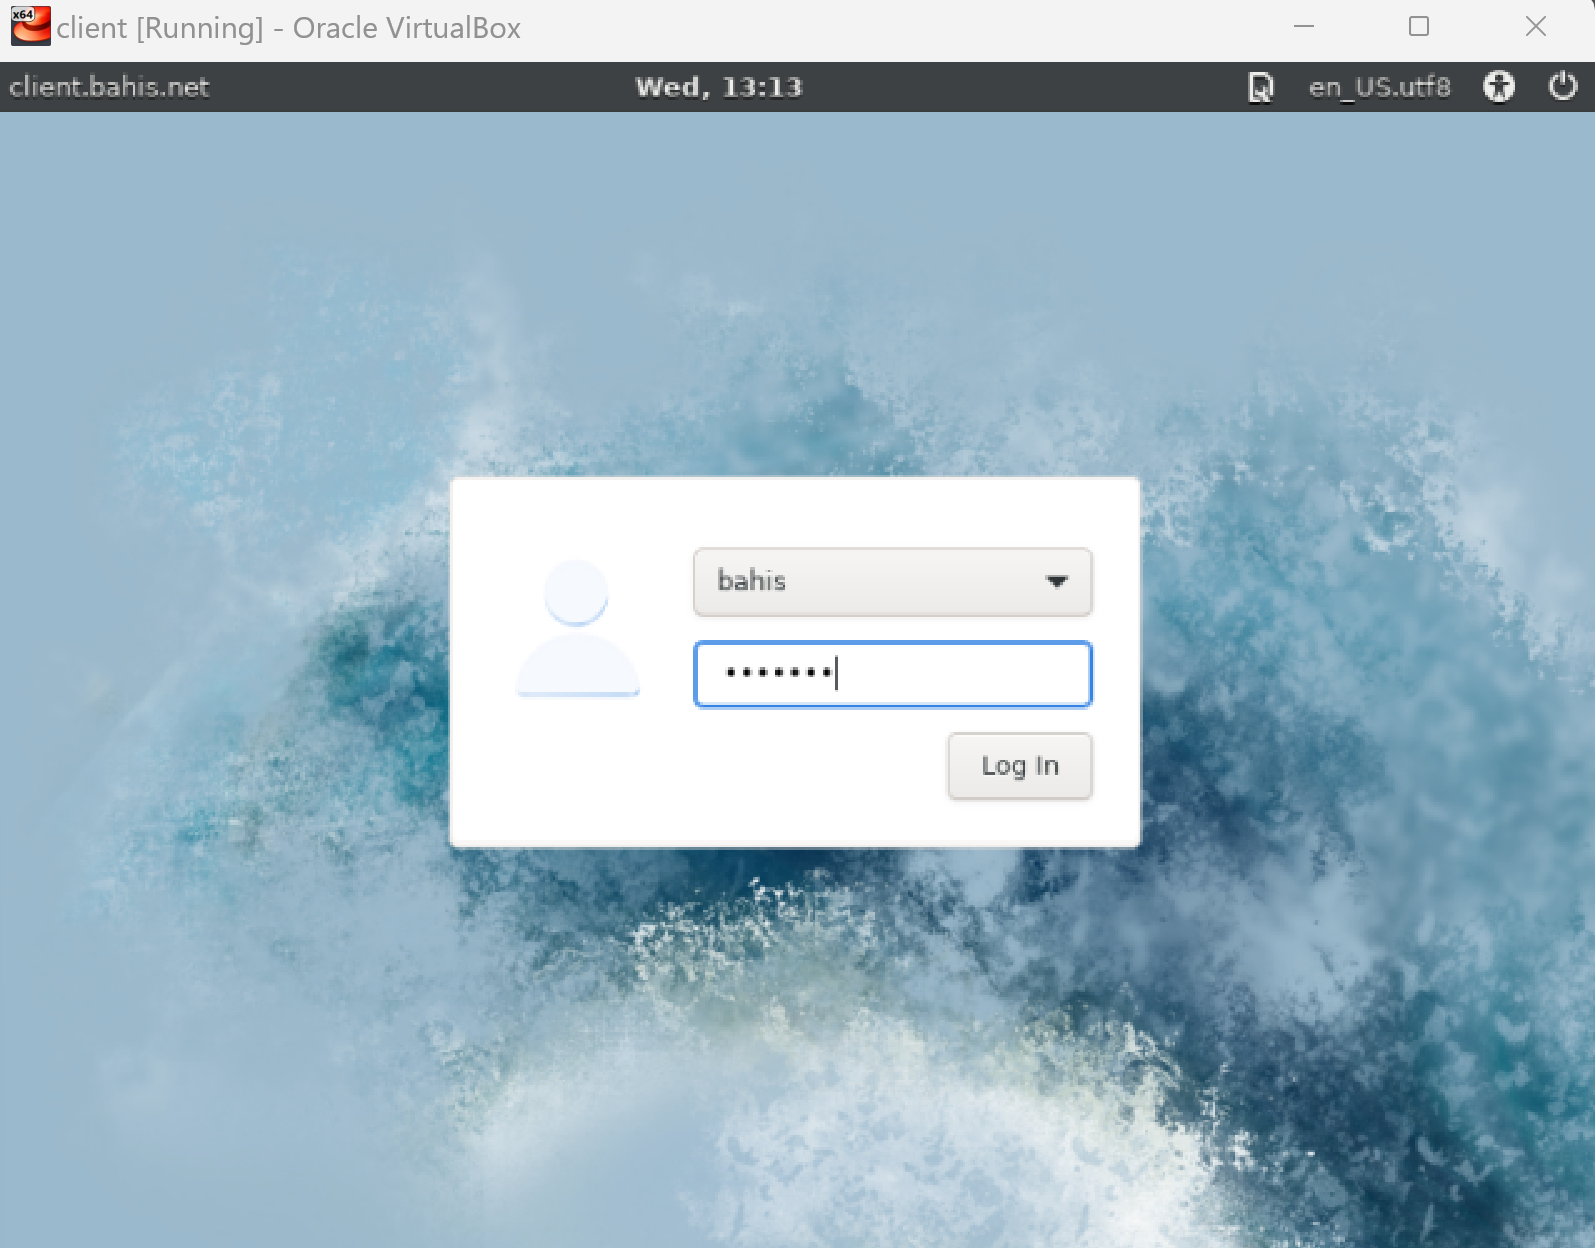
\includegraphics[width=0.7\linewidth,height=\textheight,keepaspectratio]{image/23-1.png}
\href{https://github.com/ArsenioPacavira99/study_2025-2026_net-os-admin-12/tree/master/labs/lab01/report/image/23-1.png}{рис.
23-1} !{[}Проверка SSH-подключения и отображения приглашения
пользователя{]}

\chapter{Выводы}\label{ux432ux44bux432ux43eux434ux44b}

В ходе работы выполнена автоматическая сборка box-файла Rocky Linux с
использованием Packer и его регистрация в Vagrant. Развёрнуты
виртуальные машины server и client, применены provisioning-скрипты для
создания пользователя и настройки hostname. Подтверждена корректная
работа SSH-доступа и сетевых параметров. Лабораторный стенд в ОС Windows
успешно подготовлен к дальнейшей работе.

\chapter{Контрольные
вопросы:}\label{ux43aux43eux43dux442ux440ux43eux43bux44cux43dux44bux435-ux432ux43eux43fux440ux43eux441ux44b}

\begin{enumerate}
\def\labelenumi{\arabic{enumi}.}
\item
  Для чего предназначен Vagrant? -- Это инструмент для создания и
  управления средами виртуальных машин в одном рабочем процессе. Он
  позволяет автоматизировать процесс установки на виртуальную машину как
  основного дистрибутива операционной системы, так и настройки
  необходимого в дальнейшем программного обеспечения.
\item
  Что такое box-файл? В чём назначение Vagrantfile? - box-файл (или
  Vagrant Box) --- сохранённый образ виртуальной машины с развёрнутой в
  ней операционной системой, box-файл используется как основа для
  клонирования виртуальных машин с теми или иными настройками.
  Vagrantfile --- конфигурационный файл, написанный на языке Ruby, в
  котором указаны настройки запуска виртуальной машины.
\item
  Приведите описание и примеры вызова основных команд Vagrant. vagrant
  help --- вызов справки по командам Vagrant; vagrant box list ---
  список подключённых к Vagrant box-файлов; vagrant box add ---
  подключение box-файла к Vagrant; vagrant destroy--- отключение
  box-файла от Vagrant и удаление его из виртуального окружения; vagrant
  init --- создание «шаблонного» конфигурационного файла Vagrantfile для
  его последующего изменения; vagrant up --- запуск виртуальной машины с
  использованием инструкций по запуску из конфигурационного файла
  Vagrantfile; vagrant reload --- перезагрузка виртуальной машины;
  vagrant halt --- остановка и выключение виртуальной машины; vagrant
  provision --- настройка внутреннего окружения имеющейся виртуальной
  машины (например, добавление новых инструкций (скриптов) в ранее
  созданную виртуальную машину); vagrant ssh --- подключение к
  виртуальной машине через ssh.
\item
  Дайте построчные пояснения содержания файлов vagrant-rocky.pkr.hcl,
  ks.cfg, Vagrantfile, Makefile. Vagrantfile - Первые две строки
  указывают на режим работы с Vagrantfile и использование языка Ruby.
  Затем идёт цикл do, заменяющий конструкцию Vagrant.configure далее по
  тексту на config. Строка config.vm.box = \enquote{BOX\_NAME} задаёт
  название образа (box-файла) виртуальной машины (обычно выбирается из
  официального репозитория). Строка config.vm.hostname =
  \enquote{HOST\_NAME} задаёт имя виртуальной машины. Конструкция
  config.vm.network задаёт тип сетевого соединения и может иметь
  следующие назначения: -- config.vm.network \enquote{private\_network},
  ip: \enquote{xxx.xxx.xxx.xxx} --- адрес из внутренней сети; --
  config.vm.network \enquote{public\_network}, ip:
  \enquote{xxx.xxx.xxx.xxx} --- публичный адрес, по которому виртуальная
  машина будет доступна; -- config.vm.network
  \enquote{private\_network}, type: \enquote{dhcp} --- адрес,
  назначаемый по протоколу DHCP. Строка config.vm.define
  \enquote{VM\_NAME} задаёт название виртуальной машины, по которому
  можно обращаться к ней из Vagrant и VirtualBox. В конце идёт
  конструкция, определяющая параметры провайдера, а именно запуск
  виртуальной машины без графического интерфейса и с выделением 1 ГБ
  памяти.
\end{enumerate}

\chapter{Список
литературы}\label{ux441ux43fux438ux441ux43eux43a-ux43bux438ux442ux435ux440ux430ux442ux443ux440ux44b}

\begin{enumerate}
\def\labelenumi{\arabic{enumi}.}
\item
  GNU Bash Manual. --- 2019. --- URL:
  https://www.gnu.org/software/bash/manual/ (дата обр. 13.09.2021).
\item
  GNU Make Manual. --- 2016. --- URL:
  http://www.gnu.org/software/make/manual/ (visited on 09/13/2021).
\item
  Powers S. \emph{Vagrant Simplified {[}Просто о Vagrant{]}} / Пер.: А.
  Панин // Библиотека сайта ruslinux.net. --- 2015. --- URL:
  http://rus-linux.net/MyLDP/vm/vagrant-simplified.html (visited on
  09/13/2021).
\item
  Vagrant Documentation. --- URL: https://www.vagrantup.com/docs
  (visited on 09/13/2021).
\item
  Купер М. \emph{Искусство программирования на языке сценариев командной
  оболочки}. --- 2004. --- URL:
  https://www.opennet.ru/docs/RUS/bash\_scripting\_guide/ (дата обр.
  13.09.2021).
\end{enumerate}


\printbibliography



\end{document}
